\section{\uppercase{Experiments and Results}}
\label{sec:experiments}

\noindent
In order to show the effectiveness of RALA-ChangeFormer, we evaluate our proposal on two widely used benchmarks. Our experiments assess both segmentation accuracy and computational efficiency after replacing the quadratic MHSA modules of ChangeFormer with the RALA mechanism. All comparisons are made against the original ChangeFormer \cite{Bandara2022ChangeFormer}.

\noindent \textbf{LEVIR-CD.} LEVIR-CD \cite{Zheng2020LEVIR} contains 637 bi-temporal high-resolution image pairs (1024$\times$1024) depicting building changes in rapidly developing urban areas. Following standard practice, each pair is cropped into non-overlapping 256$\times$256 tiles, yielding: \text{Train/Val/Test} = 6096 / 762 / 762.

\noindent \textbf{DSIFN-CD.} DSIFN-CD \cite{Shen2021DSIFN} includes multi-class land-cover and building change scenes under heterogeneous imaging conditions. Each 512$\times$512 pair is divided into non-overlapping 256$\times$256 tiles, producing: \text{Train/Val/Test} = 14400 / 1360 / 192.

Ground-truth labels in both datasets are binary change masks. For efficiency experiments, the following is added (i) input patch resolution, and (ii) batch size until GPU out-of-memory (OOM) is reached.

\noindent \textbf{Implementation Details.} All experiments are implemented in PyTorch, matching the software environment used by the ChangeFormer implementation \cite{Bandara2022ChangeFormer} for fair comparison.

For \textbf{LEVIR-CD}, both ChangeFormer (CF) and RALA-ChangeFormer (RALA-CF) are initialized from the SegFormer-B2 encoder pretrained on ADE20K, following the training protocol of the original ChangeFormer~\cite{Bandara2022ChangeFormer}. An initial learning rate with cosine decay of $1\times10^{-4}$ is used.

For \textbf{DSIFN-CD}, CF is fine-tuned from the best CF checkpoint obtained on LEVIR-CD using a reduced learning rate of $6\times10^{-5}$. Analogously, RALA-CF is initialized from the best RALA-CF checkpoint trained on LEVIR-CD and optimized under the same schedule. In all experiments, the only architectural difference between CF and RALA-CF lies in the encoder attention modules (standard MHSA vs.\ rank-augmented linear attention).


\subsection{Evaluation Metrics}

We report standard change detection metrics following the state-of-the-art BCD models \cite{Zheng2020LEVIR, Shen2021DSIFN, Bandara2022ChangeFormer, Chen2022BIT, Fang2021SNUNetCD}. To measure computational efficiency, we additionally track (a) total learnable parameters, (b) GFLOPs per forward pass, (c) peak GPU memory consumption, (d) maximum feasible batch size before OOM and (e) training throughput (images/s).

\noindent \textbf{Results on Segmentation Accuracy}

\begin{table}[h!]
\caption{Segmentation accuracy of baseline BCD models and our variants on LEVIR-CD and DSIFN-CD using $256\times256$ input patches and batch size 16. 
Metrics for SNUNet-CD and BIT are taken from the original ChangeFormer paper \cite{Bandara2022ChangeFormer}.}
\label{tab:accuracy}
\centering
\resizebox{\columnwidth}{!}{
\begin{tabular}{lcccc}
\hline
\textbf{Model} & \textbf{Dataset} & \textbf{F1} & \textbf{IoU} & \textbf{OA} \\
\hline
SNUNet-CD~\cite{Fang2021SNUNetCD} & LEVIR-CD & 88.16 & 78.83 & 98.82 \\
BIT~\cite{Chen2022BIT}            & LEVIR-CD & 89.31 & 80.68 & 98.92 \\
CF~\cite{Bandara2022ChangeFormer} & LEVIR-CD & 90.40 & 82.48 & 99.04 \\
\rowcolor{pastelorange}
RALA-CF (ours) & LEVIR-CD & \textbf{89.87} & \textbf{81.60} & \textbf{98.99} \\

\hline
SNUNet-CD~\cite{Fang2021SNUNetCD} & DSIFN-CD & 66.18 & 49.45 & 87.34 \\
BIT~\cite{Chen2022BIT}            & DSIFN-CD & 69.26 & 52.97 & 89.41 \\
CF~\cite{Bandara2022ChangeFormer} & DSIFN-CD & 86.67 & 76.48 & 95.56 \\
\rowcolor{pastelorange}
RALA-CF (ours) & DSIFN-CD & \textbf{84.07} & \textbf{73.96} & \textbf{92.44} \\
\hline
\end{tabular}
}
\end{table}

\noindent As shown in Table~\ref{tab:accuracy}, RALA-CF matches the segmentation accuracy of the baseline ChangeFormer on both datasets, while outperforming prior BCD models such as BIT and SNUNet-CD. This indicates that replacing MHSA with rank-augmented linear attention preserves the segmentation capability of ChangeFormer.

\noindent \textbf{Efficiency Analysis}.

\begin{table}[h!]
\caption{Efficiency comparison between ChangeFormer and RALA-ChangeFormer ($256\times256$ inputs, batch size 16).}
\label{tab:efficiency}
\centering
\resizebox{\columnwidth}{!}{
\begin{tabular}{lccc}
\hline
\textbf{Model} & \textbf{Params (M)} & \textbf{GFLOPs} & \textbf{Peak VRAM (GB)} \\
\hline
CF & 247 & 248.77 & 27 \\
\rowcolor{pastelorange}
RALA-CF & \textbf{243} & \textbf{228.62} & \textbf{21} \\
\hline
\end{tabular}
}
\end{table}

\noindent Table~\ref{tab:efficiency} shows that RALA-CF reduces FLOPs by approximately 8--10\% and peak memory usage by \textbf{20--30}\% without altering the overall architecture. These savings translate into faster training and more flexible batch-size configurations.

\noindent \textbf{Maximum Batch Size Experiments}

\begin{table}[h!]
\caption{Maximum batch size before OOM for different input resolutions. VRAM limit: 34--36 GB (A100 40 GB VRAM GPU).}
\label{tab:batch_multires}
\centering
\resizebox{\columnwidth}{!}{
\begin{tabular}{lccc}
\hline
\textbf{Resolution} & \textbf{Model} & \textbf{Max Batch} & \textbf{VRAM at OOM (GB)} \\
\hline
\multirow{256$\times$256} 
& CF       & 32 & 34 \\
& RALA-CF  & \textbf{48} & \textbf{34} \\
\hline
\multirow{512$\times$512} 
& CF       & 8  & 34 \\
& RALA-CF  & \textbf{12} & \textbf{34} \\
\hline
\multirow{1024$\times$1024} 
& CF       & 2  & 36 \\
& RALA-CF  & \textbf{3} & \textbf{36} \\
\hline
\end{tabular}
}
\end{table}

\noindent \textbf{Ablation: MHSA vs.\ RALA}. To isolate the contribution, we perform an ablation where only encoder attention is replaced with RALA, and all other components remain unchanged.

\begin{table}[h!]
\caption{Ablation study isolating the encoder attention mechanism.}
\label{tab:ablation}
\centering
\resizebox{\columnwidth}{!}{
\begin{tabular}{lccc}
\hline
\textbf{Variant} & \textbf{GFLOPs} & \textbf{VRAM (GB)} \\
\hline
Baseline MHSA & 86.17 & 12 \\
\rowcolor{pastelorange}
Encoder: RALA & \textbf{76.95} & \textbf{8} \\
\hline
\end{tabular}
}
\end{table}

\noindent As shown in Table~\ref{tab:ablation}, most computational savings originate from replacing MHSA within the encoder, where token counts are highest and attention cost dominates.

\subsection{Discussion}
\label{sec:discussion}

The experimental results demonstrate that integrating RALA into the encoder of ChangeFormer provides consistent computational advantages while preserving segmentation accuracy in multi-temporal BCD. Since the modification affects only the encoder self-attention modules—leaving the convolutional backbone, FFN layers, and decoder head unchanged—the magnitude of improvements is moderate but systematic across all benchmarks.

\noindent \textbf{Accuracy–Efficiency Balance.}
As shown in Table~\ref{tab:accuracy}, RALA-ChangeFormer achieves nearly identical F1, IoU, and OA scores to the baseline ChangeFormer on both datasets \cite{Zheng2020LEVIR,Shen2021DSIFN}. The differences fall within normal training variance, indicating that the rank-augmented linear formulation retains the model’s ability to represent spatial–temporal interactions between bi-temporal features maps. Importantly, while many linear-attention variants \cite{Choromanski2021Performer,Wang2020Linformer,Xiong2021Nystromformer} exhibit a well-documented degradation in dense vision problems due to low-rank collapse, RALA avoids this issue by explicitly increasing the diversity of its KV buffer. This preservation of representational capacity is further illustrated by the attention maps in Fig.~\ref{fig:attn_maps}, which provide a qualitative visualization of the spatial attention distribution. Collectively, these results confirm that RALA maintains reliable prediction for this specific tasks, despite replacing quadratic attention.

\noindent \textbf{Computational Benefits and Practical Scalability.}
Table~\ref{tab:efficiency} shows clear reductions in FLOPs and peak VRAM usage when MHSA is replaced with RALA. Although iteration-level speedups are modest, the improvements compound at higher resolutions, where MHSA cost is highest. The increased feasible batch sizes (Table~\ref{tab:batch_multires}) highlight the most practical advantage: RALA-CF can process substantially more images per iteration under identical hardware constraints. In the context of remote sensing, where datasets may contain tens or hundreds of thousands of patches, this translates into significantly higher throughput and faster experimentation cycles. Moreover, training with larger batches allows exposure to more diverse samples per step, improving stability and enabling efficient learning on large, out-of-distribution datasets. In contrast, baseline MHSA-based architectures often require prohibitively small batches that impair convergence behavior on heterogeneous datasets such as DSIFN-CD.

\noindent \textbf{Encoder-Level Efficiency Gains.}
The ablation in Table~\ref{tab:ablation} isolates the source of the computational savings, showing that almost all reductions originate from the encoder, where token density is highest and attention cost dominates. The decoder contributes marginally to computational load, so modifying only the encoder yields the majority of benefits while maintaining full architecture compatibility.

In summary, RALA-ChangeFormer achieves meaningful efficiency gains without compromising segmentation quality, while offering practical scalability advantages for high-resolution or large-scale BCD pipelines under fixed GPU memory budgets.

\begin{figure}[t]
    \centering
    \begin{subfigure}{0.48\linewidth}
        \centering
        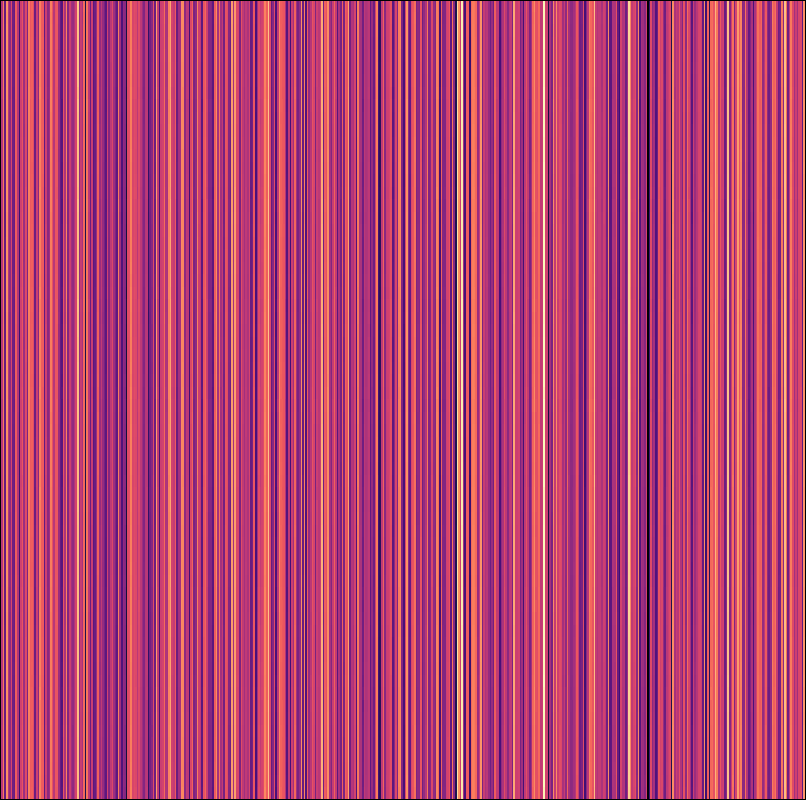
\includegraphics[width=\linewidth]{images/Attention_Map_CF.pdf}
        \caption{CF (MHSA).}
        \label{fig:attn_cf}
    \end{subfigure}
    \hfill
    \begin{subfigure}{0.48\linewidth}
        \centering
        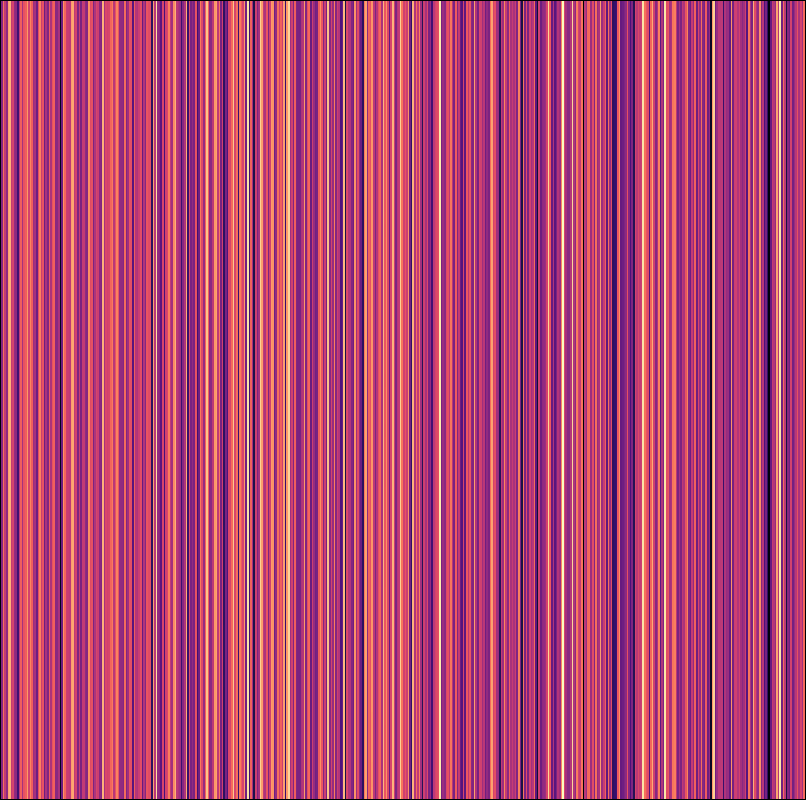
\includegraphics[width=\linewidth]{images/Attention_Map_RALA_CF.pdf}
        \caption{RALA-CF (RALA).}
        \label{fig:attn_rala}
    \end{subfigure}
    \caption{Token-wise attention maps at the last encoder stage
    ($N{=}512$ tokens on the x-axis, $d{=}64$ channels on the y-axis) for the baseline ChangeFormer and the proposed RALA-ChangeFormer.
    Colors represent normalized attention intensity, where darker values indicate low attention response and brighter (purple) values indicate higher attention. The maps are shown for qualitative comparison only, illustrating that RALA preserves non-collapsing spatial attention patterns comparable to MHSA.}
    \label{fig:attn_maps}
\end{figure}

\subsection{Limitations}
\label{subsec:limitations}

Despite the advantages demonstrated in Sections~\ref{sec:experiments} and~\ref{sec:discussion}, the proposed integration of rank-augmented linear attention exhibits several limitations that contextualize its practical impact.

\noindent \textbf{(1) Moderate end-to-end computational gains.} Although rank augmentation substantially reduces the cost of encoder self-attention, the overall computational footprint of ChangeFormer is still influenced by multiscale fusion layers. As shown in Table~\ref{tab:efficiency}, the reduction in total GFLOPs remains moderate (8--10\%), since attention constitutes only part of the complete pipeline.


\noindent \textbf{(2) Efficiency improvements grow with token count.} RALA provides the largest benefits when the number of tokens is high (e.g., 512 or 1024 resolution). At lower input sizes such as $256\times256$, improvements are measurable but less pronounced, which limits impact for applications operating strictly at small patch resolutions.

\noindent \textbf{(3) Limited impact on model expressiveness beyond attention.} While RALA mitigates the low-rank collapse common in linear attention and preserves segmentation performance, it does not enhance the expressive capacity of non-attention modules such as convolutional encoders or decoder fusion layers. As a result, the overall accuracy remains bounded by the representational capacity of the original ChangeFormer architecture.

\noindent \textbf{(4) Limited evaluation on independent acquisition domains.}
The experimental evaluation follows the standard training and testing protocols of LEVIR-CD and DSIFN-CD, where splits are spatially disjoint but not fully independent in terms of acquisition conditions or geographic regions. While this work focuses on computational scalability and efficiency under commonly adopted BCD benchmarks, the generalization of RALA-ChangeFormer to unseen acquisition domains (e.g., cross-region or cross-sensor settings) remains an open question. Evaluating rank-augmented linear attention under fully independent data distributions is a promising direction for future work.

\medskip
\noindent  Overall, although the proposed integration offers practical advantages in memory efficiency, scalability, and batch-size flexibility, it does not eliminate the structural constraints inherent to hierarchical encoder--decoder architectures. These considerations frame the scope of improvements achieved by substituting MHSA with rank-augmented linear attention.
